\chapter{Background}
\label{chap:background}

Previous studies have used fine-grain instrumentation to dive into previously inaccessible student behaviors. These studies varied widely, from the discovery of phases of development over a project \citep{berland-2013, martin2013nanogenetic}, to analysis of off-task behavior in learning \citep{baker2004off}. Some have presented methods for identifying struggling students \cite{piech-2012}, and others develop well-informed assessments \citep{werner2012fairy}. All of them had commonalities: building models of learning by looking at fine-grain behavior data, observing small changes in work over time, filling in the stories that led up to the final artifacts. Examining the process of programming rather than the final products can uncover interesting behavior about student learning, and such patterns may have better predictive power than in-class exams \citep{blikstein2014}.

Analysis of this data was informed by previous studies of student behavior in programming, math, and other activities. \cite{perkins-1986} identified and classified types of behaviors students exhibit when they encounter difficulty in programming. Off-task behavior, to which flailing may be related, has also been studied, such as \cite{baker2004off} did, in the context of mathematics. 

This study relates closely to learning pathways, especially those identified by learning analytics \citep{martin2013nanogenetic}. 

The activities conducted for data collection revolved around debugging, as debugging has been shown to be a compelling mechanism to drive engagement with a short programming task \citep{webb2010troubleshooting}.

A more extensive discussion of related work is presented below.


% \section{A Brief History of Learning Theory}
% \label{sec:learning-theory}
% Piaget, ZPD, etc etc
% Also introduce Orchestration
% ...
% Maintaining each students' current position within their zone of proximal development is a critical goal of orchestration, which will be further discussed in Section \ref{sec:teacher-dashboards}.
%TODO this is a stub


\section{Visual Languages}
\label{sec:visual-languages}

Much of the literature concerning programming efficacy was done at a time when visual languages were emerging as a purported panacea of usefulness \citep{shu-1988}, but with little empirical evidence to substantiate those claims \citep{petre-1995}. \citeauthor{sch-1980} made such an accusation, ``Computer scientists... make broad claims for the simplicity, naturalness, or ease-of-use of new computer languages or techniques, but do not take advantage of the opportunity for experimental confirmation'' (\citeyear{sch-1980}). \citeauthor{stefik2014programming} strongly argued that these ``language wars'' are a significant problem to science, and as stewards of computation, it is the language researchers who must study the impact of language designs on people (\citeyear{stefik2014programming}). Speaking of diagram-based visual languages, \citet{blackwell-2001} offered a challenge to researchers to support their claims of intuition through visual programming, ``...to explain why this intuition may be valid, and to propose the ways in which, if it is valid, it can most be effectively exploited.'' This work hopes to shed some light into the domain illustrated by that challenge. 


\section{App Inventor}
\label{sec:app-inventor-background}
App Inventor is an online development environment to build Android apps, employing a drag-and-drop designer and graphical, blocks-based code editing. App Inventor follows in the tradition of Constructionism \citep{papert1991situating}, which covers a wide class of discovery-based pedagogical vehicles. App Inventor is also deeply influenced by Scratch \citep{resnick2009scratch}, and offers low barriers for entry, high ceilings of capability, and a built-in library of powerful abstractions.

The App Inventor language and runtime uses a purely event-driven programming model, where all functions are driven by events and event handler code \citep{turbak-2014}. The event handlers are separate blocks, and can be organized arbitrarily on the workspace. An example of two event handlers can be seen as the gold, top-level blocks in Figure \ref{fig:debug0ch2}. 

\begin{figure}
  \centering
      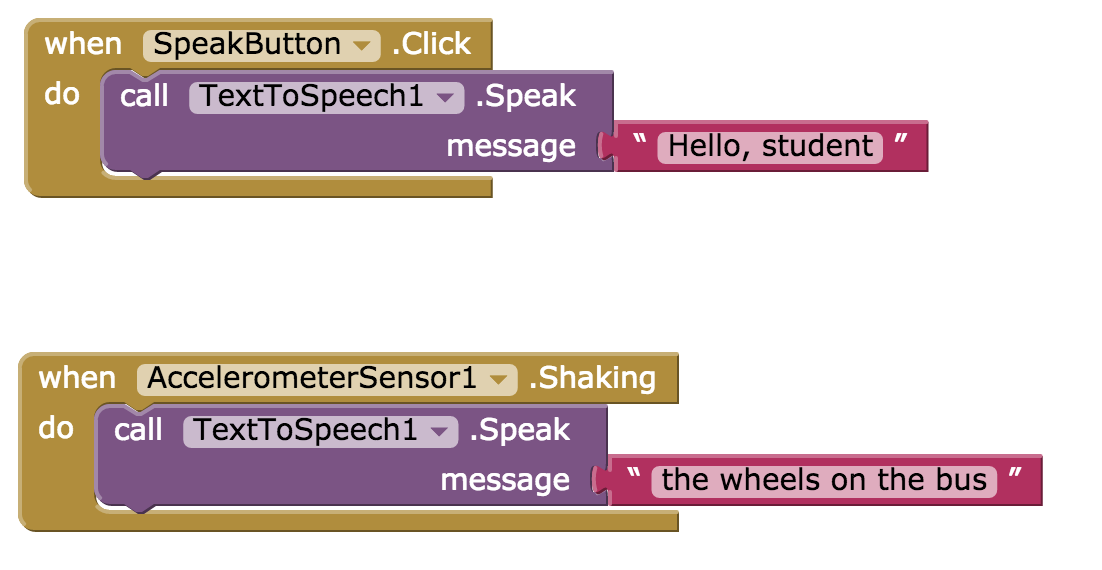
\includegraphics[width=\textwidth]{images/debugActivity/debug0start}
  \caption[Some App Inventor code blocks]{Some App Inventor code blocks. Each gold-colored block is an event handler, which can be arranged arbitrarily on the workspace. The enclosed purple blocks will execute when their parent events are triggered.}
  \label{fig:debug0ch2}
\end{figure}


% \section{Cognitive Dimensions of Notations} 
% \label{sec:CDs}
% The Cognitive Dimensions of Notations framework was developed to provide a vocabulary through which design tools can be assessed and discussed. This framework is suitable for broad evaluation and discussion of how a language suits its users needs. It was developed over many years \citep{green1989cognitive, green1996usability}, and is currently canonized in \citet{blackwell-2003}. Their mission was for this vocabulary to be easily applicable, understandable, and most importantly, be theoretically coherent \citep{petre-2006}. 

%The cognitive dimensions framework presented an empirically-derived set of dimensions that can be generally measured for a given class of user activity. These dimensions described different cognitive mechanisms that are necessary for the user to execute a given action, and helped create a meaningful dialog about how those dimensions can be traded to optimize the action for the user \citep{blackwell-2003}. The research was started to investigate why some notations work and don't work for the people using them \citep{petre-2006}. 

%The dimensions alone do not constitute anything. A dimension is not good or bad. Dimensions are part of the framework's instrument, which includes evaluation of relevant dimensions for a particular task. Application of the the dimensions to a set of representative tasks is what drives the apparatus, and the assessment is in the comparison of the desired dimensionality for those tasks compared to the observed value of those dimensions for the task. This also makes it possible to use the cognitive dimensions framework, in a constrained form, as a user survey tool, to provide users with a method for describing their experience with a notation system.

%Without any further fanfare, here are the dimensions, in their entirety as of \citeyear{blackwell-2003}:
% The dimension most critical to this work was \emph{secondary notation,} the information encoded in means other than the formal syntax, primarily in graphical layout. Secondary notation is explored further in Section \ref{sec:secondary-notation} Additionally, \emph{viscosity,} the difficult to make a change, was relevant to this study.

% \begin{description}
% \item [Viscosity] Resistance to change, or difficulty to make a change. Modifying heading styles across a document manually is a viscous activity, in that the user's desired action is seemingly simple, but the effort to execute it is significant.
%\item [Visibility] Ability to view components easily. This dimensions is often traded away in languages in favor of, for example, abstractions.
%\item [Premature commitment] Constraints placed on the order of doing things. In programming, a mechanic of premature commitment forces the programmer to make decisions before they have the information to base the decision on. \citet{roast-2000} described this as "the user having to satisfy the secondary goal prior to achieving the primary goal."
% \item [Hidden dependencies] Entities may cite each other, and a change in one entity may create change elsewhere unexpectedly due ot unapparent citations. This is common in spreadsheets, where cell references are not easily visible.
%\item [Role-expressiveness] The purpose of an entity is readily inferred. The reader can discover the author's intent. 
%\item [Error-proneness] Invites mistakes. Can be protected with preventative mechanisms.  
%\item [Abstractions] Change the underlying notation. Common examples are macros, functions, global find-and-replace, word processor styles, and even speed dial. They can be persistent (macros) or transient (find and replace). An abstraction manager is necessary if the user is allowed to edit the abstractions. 
% \item [Secondary notation] Information encoded in means other than the formal syntax. 
%\item [Closeness of mapping] How closely the notation relates to the result it describes. 
%\item [Consistency] Similar semantics are expressed in similar syntactic forms. Information can be obscured by inconsistent presentation.
%\item [Diffuseness] Verbosity of the language. Large icons, long phrases, and other forms of graphical real estate consumption contribute to diffuseness. I do not know why this dimensions isn't called verbosity, which could easily be contrasted by calling low verbosity succinct.
%\item [Hard mental operations] Creates high demand on cognitive resources. This is an interesting dimension, as it makes clear to designers that sometimes a notation can force a user to work things out in their head, or otherwise tax working memory.
%\item [Provisionality] Provisional notation, meaning temporary, allows for low commitment to a notation. This may be useful for sketching, recording potential options, ``what if'' exercises, and general exploration activities.
%\item [Progressive evaluation] Work can be checked at any time. Evaluation is an important part of the design process, and drives iteration \citep{atman-2003}. A well-known advantage to interpreted programming environments is their ease of work evaluation, where the user can try out partially-completed programs at any time, and have meaningful interactions with their partial work.
% \end{description}


% \subsection{Secondary Notation}
% \label{sec:secondary-notation}
% One of these dimensions in particular, secondary notation, emerged as especially important to visual programming \citep{petre-2006}. The work at the time was focused on diagram programming, such as LabVIEW, where researchers found a distinct and repeating signal that differentiated experts from novices. That signal was in the use of secondary notation, where experts would use arrangement and layout of the diagram itself to convey information not encoded in the formal notation. 

% Secondary notation is, generally, any notation that's not part of the formal notation, and may include comments and whitespace in text languages, layout in diagrams, proximity in blocks languages, and much more. Often, secondary notation can be used however the user likes, and therefore can be used to record information that the designer of the notation did not anticipate. \citet{petre-1995} claimed that much of the comprehensibility of graphical programming is in the secondary notation, and \citet{raymond-1991} conjectured, even earlier, that the layout of a visual program was the most important, and possibly only, aspect that was truly visual. Of course, \citeauthor{raymond-1991} had a very specific meaning of ``visual,'' where it depended on being non-discrete, unable to guarantee syntactic or semantic differentiation, similar to the mathematical notion of continuity or the electronic notion of analog. In fact, \citeauthor{raymond-1991} called such a language Analog, and contrasted it against Notational languages, which were discrete, with strongly differentiable notational marks and strongly differentiable conceptual objects being represented. This distinction of Notational versus Analog language was developed earlier as part of an interesting philosophical discussion on notations, and asked hard questions about denotation and representation \citep{goodman-1976}. This discussion had nothing to do with programming, nor visual programming, but it was brought into that domain by \citeauthor{raymond-1991}, and nearly predicted the findings of the expert and novice usage difference in secondary notation, found later by \citet{petre-2006}.

\section{Behaviors when Encountering Difficulty}
\label{sec:behaviors}
Novice programmers are faced with a plethora of difficulties to overcome. \citet{perkins-1986} identified some key behavior patterns students may show when they encounter difficulty. To begin, \citeauthor{perkins-1986} observed that most students displayed ``significant powers of invention'' when working with programming tasks, and they employed that inventiveness in tackling problems they encountered. However, there were are an enormous number of pitfalls in the programming process that interfered with that inventiveness leading to a reasonable degree of competence. 

The general behavior patterns that \citet{perkins-1986} identified are as follows. There were two conceptual cohorts: \emph{stoppers} and \emph{movers.} When a stopper found themselves without an immediate answer to a difficulty, they felt at a complete loss, and were unwilling to further explore the problem. They would completely stop working, often sitting back from the computer. This behavior is extremely common, and has been personally observed by the author. A stopper can be rescued with immediate intervention, where a teacher can assess and ask the next questions explicitly (such as ``what do you think that error means?''), and press the student for answers. With this sort of intervention, stoppers usually found a solution for their difficulty, and were able to resume. In the observations of \citeauthor{perkins-1986}, the activities were short, so a rescued stopper could make it successfully to the end of the activity with only one intervention. But that intervention was timely, asserted immediately when the student stopped progressing, which allowed the researcher to re-direct the student without a loss of context. Such an intervention in a regular classroom would require a large amount of teacher time per student. Outside of a research environment, this could be difficulty to reliably achieve.

Opposite of the stoppers were the movers, who were identified by a collection of traits, pivoting around the lack of fear to try things, and the lack of frustration if things do not work. Movers consistently tried one idea after another, and never stopped long enough to appear to be stuck. This may sound like a generally desirable behavior pattern over the stoppers, but the movers also had difficulties. Extreme movers moved too fast, modifying without reflection, resulting in changes to their code that clearly did not work. These extreme movers did not appear to draw lessons from their failed ideas, nor did they display behavior of honing in towards a solution. They appeared emotionally distant from the task, where \citeauthor{perkins-1986} conjectured that the keyboard and screen served as a ``handy distraction,'' allowing students to keep themselves busy without having to stop and think. The author claims this behavior to be akin to \emph{fidgeting,} although \citeauthor{perkins-1986} did not use that term. An extreme mover may actually be a stopper, we reason, but instead of acknowledging their seemingly insurmountable barrier, they fidget with their code until time expires.

\citet{perkins-1986} further expanded on a specific behavior of a mover, \emph{tinkering.} This word is often associated with tools that are intentionally friendly to discovery through experimentation and bottom-up design, such as Scratch \citep{resnick2009scratch}. \citeauthor{perkins-1986} maintained a more sterile definition, devoid of positive or negative connotation--- tinkering is simply the behavior of making many small changes to a program in hopes of getting it to work. This bottom-up behavior can be considered \emph{bricolage}, where a programmer can recruit a plethora of options from a menu and then assemble them completely experimentally, with no predrawn plan \citep{turkle1990epistemological, strauss1962savage}. This method of interaction and discovery is beneficial for early learning \citep{turkle1992epistemological}, but is not without criticism towards how it effects future, more advanced computer science learning \citep{Meerbaum-Salant:2011:HPS:1999747.1999796}.

In the observations of \citeauthor{perkins-1986}, tinkering sometimes presented a decidedly negative pattern, where the student wrongly assumed that some minor change was required to achieve their goal, and did not engage in deep thought about the problem. This was often seen alongside poor tracking skills, where the student did not follow what the code they were writing would actually do. The student never stopped to question their understanding of how the program, or the machine under it, worked.

The skill of questioning one's own understanding could be considered advanced. Executing ``good tracking,'' as \citet{perkins-1986} put it, actually relies on an understanding beneath the code syntax. The concept of the \emph{notional machine,} as introduced by \citet{duboulay-1986}, describes the underlying mechanism of the programming language that students are truly attempting to master. \citeauthor{duboulay-1986} observed that the notional machine is usually not taught at all, with attention instead going to the syntax and structure of language, without concern for the device it represented. \citeauthor{duboulay-1986} intended to empower educators with the notional machine, and encouraged teachers to build their pedagogy to expose it. 

The worst case of tinkering was observed when students accumulated multiple untested changes, or did not remove failed changes, which eventually rendered the problem incomprehensible. Any computer science instructor has likely seen the end result of such a pattern. But tinkering in this understanding can be effective. \citeauthor{perkins-1986} used an analogy from a nearby domain. A tinkerer can easily become stuck in a local maximum, where the solution appears to be close at hand, but is actually not obtainable without significant rework. In this case the student was at the top of a small hill, the wrong hill, and would need to climb back down that hill, and up a better hill that could go higher. This was identified as a particularly tempting and insidious pattern- when a program appears to be nearly correct, but in reality requires work greater than a series of small modifications. If a student was on the correct hill, where the local maximum was also the global maximum and goal, then tinkering could be effective, if done systematically. That maximum still needed to be found, even if it was nearby. In App Inventor, there has been no study yet that tests if students behave in this way, and such insights may be uncovered during this study.

%Comparing that school of thought to the Lifelong Kindergarten's tinkering in Scratch, it first appears inconsistent. It is possible, however, that Scratch, and other constructionist learning environments, always put students on the correct hill. This could be done by heavy restriction of the domain, such as the intentionally narrow activities of Code.org. More so, they may be so well optimized for bottom-up design practices that there are no hills. Local maxima would be nearly impossible, as the goal state, and global maximum, are being defined by the student progressively as they work up towards it. 


\section{Hypothetical Causes for Flailing Behavior}
%TODO this paragraph must belong somewhere...

A student's degree of comfort in the classroom has been shown to be factor in CS1 undergrad success \citep{wilson-2002}. Comfort level was measured by a collection of factors, revolving around likelihood to ask questions (demonstrating comfort) and signs of anxiety (demonstrating discomfort). That study also found a significant factor was \emph{attribution to luck,} but it was a negative parameter. Many students, for reasons unclear, blamed their successes or failures on the unstable attribute of luck. Whether they chose to do this for failure or success correlated with different mental attitudes towards their self-efficacy. If a student was unhappy with their score, and attributed their failures to luck, it provided motivation to continue trying. However, attribution to luck in either direction had a strong negative impact on their scores ($p=0.233$). This may be a parameter that contributes to the flailing behavior, as it could be interpreted as not taking responsibility for the success or failure of the program. 

Another behavior pattern that intersects with flailing is ``Gaming the system.'' This behavior has been observed in students using intelligent tutoring or feedback systems, where students tried to abuse the system itself, within its rules, to achieve a correct answer without engaging with the educational material \citep{baker2004off}. This behavior showed a strong effect on learning outcomes, even when controlled for the student's previous knowledge. Discussion on why this gaming behavior emerged revolved around the student's focus on performance outcome rather than learning. Playing the game to win the points, and not to learn the content in the game, may have resulted a desire to ``gaming the system,'' to succeed at the task without succeeding in the mission of the task. This mindset of performance has been correlated with \emph{executive help seeking} behavior, where students ask for help immediately without first engaging with or attempting to solve the problem \citep{arbreton1998student}. That behavior bore resemblance both in outcome and motivation to system-gaming, and \citeauthor{baker2004off}~asserted both may be related to learned helplessness, which carries a characteristic of mis-attribution of failures. Many ``helpless'' students mis-attributed their early failures to a lack of aptitude, as a personal trait, and then avoided difficult challenges and learning opportunities \citep{dweck1988social}. 

Both \citeauthor{wilson-2002} and \citeauthor{baker2004off} propose mis-attributions of failure and success as strong parts of a students' motivation to engage or disconnect with a problem. In this study, students could do both--- flailing appeared to be on-task, but uninformed. The question of the student asks themselves as to how to approach a problem when stuck will require further work. This sort of mis-attribution, both personally and socially, is interesting to the author.

Students working in App Inventor have often been observed doing unproductive tinkering, similar to that observed by \citet{perkins-1986}. One hypothesis as to why App Inventor does this can be made with the help of the Cognitive Dimensions Framework \citep{blackwell-2003}. As \citet{petre-2006} observed, experts and novices write and read secondary notation in different ways, and in App Inventor, poor planning of that secondary notation by a novice can result in increased viscosity. Increased viscosity, we hypothesize, may result in tinkering behavior, as it adds time and cognitive load to the user's task. Further investigation along this line is reserved for future work.


\section{Programming Environment Instrumentation}
Building instrumentation into an IDE is a method to ``get inside'' the process students go through while programming. Such instrumentation can capture a vast number of intermediate states of an assignment, allowing researchers to see the process that went into a product, instead of having to conjecture based purely on the final artifacts. The idea is decades old \citep{spohrer1985goal}, but has shown significant growth in the last five years. One current and ongoing project is Blackbox, a repository of instrumented activity collected from instances of the BlueJ IDE, which has taken the concept to a worldwide scope \citep{brown2014blackbox}. Much of the recent growth of instrumentation is likely due to increased ubiquity of high-speed Internet and online development environments. In these environments, of which App Inventor is one, programming is done in a browser application, so the entire environment is already working in concert with a central server. This model makes data collection easier than the typical programming model where the user's environment is installed natively on their system. Collecting data from locally installed applications, which could vary from person to person, and then transmitting to a central server is more difficult. As an example, both \citet{piech-2012} and \citet{brown2014blackbox} overcame this difficulty by enforcing one specific version of an IDE be used by all students, a constraint that standardized teaching and brought their environment models closer to the centralized, uniform one that App Inventor already enjoys.

\citet{piech-2012} took a very straightforward approach to generating in-progress data. They modified the development environment used in a CS1 course to take a \emph{snapshot} every time the student compiled their code. This snapshot was a complete version of the program at that time. Every snapshot was committed to a local git repository, so that at the end of the assignment the repository contained a full history of the project's code, from the very first words typed to completion. Recording snapshots on every save was a logical choice, as it was a good indication that the student had something they deemed ready for evaluation. \citet{lipman-phd} did similarly with his instrumentation in LearnCS, where snapshots were captured to a git repository on every save and run (where run effectively included compile). These studies looked at projects in Java and C respectively, which are languages that use the same write-compile-run model. Other languages, such as App Inventor, do not, and require different semantics as to when a snapshot should be triggered.

An additional source of instrumentation work is the field of Intelligent Tutoring Systems (ITS). These systems do not try to be fully-featured programming environments, instead providing a constrained, problem-specific environment to provide automated and useful feedback for students. These systems are typically constrained to counting submissions for a particular problem for each student, and running the specified tests for that problem. Many implementations and variations exist of this model \citep{ihantola2010review}. The data generated by this method are limited, as they do not provide insight into what the student did between submissions. \citet{sudol2012calculating} developed a more fine-grain assessment for measuring student performance of complex solving domains. These domains were nearly the same as those of this study, where correct solution were comprised of a combination of individual components. In such domains, \citeauthor{sudol2012calculating} argues, the popular ITS method of measuring student submission count and their total correctness is insufficient to properly model the student's development towards success with that activity. They further proposed a Probabilistic Distance to Solution metric, which used a Markov Model to estimate how far away the student is from the correct answer (\citeyear{sudol2012calculating}).  Such a metric can be used to detect progress over time within an activity, and can be used to inform an instructor to the current state of progress, rate of progress, and likelihood of student troubles, as will be argued in Chapter \ref{ch:discussion}.

\citet{le2007using} and \citet{mitrovic2003intelligent} are examples of more traditional ITS work, who took different approaches to develop systems that could detect the status of the students' misunderstanding, where progress towards the goal was a metric. They both carried the overhead that the problem needed to be well-constrained, and the answers to questions needed to be well-described to the analysis system. Writing such descriptions were time consuming, and the Probabilistic Distance to Solution \citep{sudol2012calculating} attempted to bring that methodology closer to to being automated, by means of a reduced need for problem-specific detail.


\section{Orchestration}
Classroom orchestration refers to the management of activities a teacher undergoes while teaching or conducting a lab session. Orchestration involves making decisions in the moment how to best apply limited resources of time, intervention assistance, technology, and the skills of other people. Teachers use orchestration skills every day. The computer lab is a particularly difficult place for orchestration, as students often work independently, unlike a lecture format, and much of the data necessary to make optimal decisions can be obscured by the computers themselves. The computer lab also is the ideal place to use technology to overcome those issues, and provide even better insight into student learning, in real time.

More formally, orchestration was defined by \citet{dillenbourg2012design} as ``how a teacher manages, in real time, multi-layered activities in a multi-constraints context." The activities span a diverse field of possible pedagogical scenarios in a classroom or lab, and it is the job of the teacher to optimize all of the factors provided by all of the tools with all the demands made by a classroom full of students. This is not the same as adaptive (or individualized) instruction, \citet{dillenbourg2012design} continued, as orchestration is at least partially open-loop and accesses variability that is extrinsic to both the teacher and student, such as the technology itself. The study of orchestration focuses not on adapting pedagogy in real time, but the regulatory processes in managing constraints of the entire environment, which then results in pedagogical adaptation decisions.

\citet{tchounikine2013clarifying} considers the "design for orchestration" concept, and provides the notion of differentiation between \emph{orchestration technology} and \emph{orchestrable technology.} An orchestration technology is technology that supports the act of orchestration, such as by providing critical information to the orchestrator. A technology that is \emph{orchestrable} is one that can be used as part of the orchestration, meaning it is adaptable in real-time to the needs of the orchestrator. The tools in this study focus on orchestration technology, enabling the teachers to know more about their students to then actuate better orchestrations. 

One tool specifically designed for teacher orchestration is AMOEBA \citep{berland2015amoeba}. AMOEBA focused on orchestration of collaboration among the students, and on the surface, aided the teacher in assigning partners for pair programming activities. It was a real-time analytics tool that determined assessed properties of the students' programming styles, which informed the teacher to better create pairings. Additionally, \citeauthor{berland2015amoeba} provided significant thought on the design principles of orchestration tools, which primarily revolve around their concept of the ``CS-ZPD,'' a zone of proximal development for computer science based on that of \citet{vygotsky1987collected}, and the theory that matched zones of proximal development is necessary for ideal partner work \citep{cooper2007effectiveness}. These principles informed the process that AMOEBA used to help choose partners, and help the teacher make good partner choices. The work on AMOEBA \citep{berland2015amoeba}was robust and thoroughly researched, and many principles from were used in this study. 


\section{Classroom Dashboards}
\label{sec:teacher-dashboards}
Classroom dashboards are a particular class of application that allows teachers to see information about their entire class of students. These are commonly found as the instructor-facing view of turn-in systems, where they report on assignments completed, attempts made, and tests passed. Many systems currently exist, and they are exciting as they provide opportunity for improved awareness, reflection, and sense-making, both for students, who can review their own work histories, and teachers, who can more easily aggregate the progress of the class \citep{verbert2013learning}. \citet{Brewer:BioBytes} developed a near real-time assessment tool for biology, based on an off-the-shelf personal response system to ``get inside'' student thinking during lectures. \citeauthor{Brewer:BioBytes} also developed a custom web-based assessment for use between lectures, which was more akin to the large-grain systems seen in computer science turn-in consoles. Faculty and staff reported improvement in student understanding of biology when using these systems (\citeyear{Brewer:BioBytes}). These systems did not work within the assignment, rather assessing a student as they progressed from lecture to lecture.

Flipped classrooms and MOOCs depend on classroom dashboards for their basic operation. The Spinoza code tutor system was an Intelligent tutoring System (ITS) for a flipped classroom model \citep{Deeb15}, where researchers added further instrumentation to detect at-risk students in CS1 courses. They found that the measures of student engagement and learning speed correlated with overall student performance \citep{Tarimo:2016:EDA:2904446.2904471}, which was an encouraging result for fine-grain analysis research. Detecting students on the verge of dropping out could be an area well-served by automated assessment systems, and would be presented by a dashboard mechanism. Flipped tools and MOOC consoles provide better insights into student learning, as the course content can be designed to depend on automation from the outset, even if that creates new pedagogical challenges \citep{Martin:2012:MOO:2240236.2240246}.

\citet{Diana:2017:IDR:3027385.3027441} posited that as learning analytics becomes more commonplace, a challenge will arise that the amount of log data will become more difficult to process, display, and interpret. They built a system to analyze student programming states at various points throughout the course, and used these data to generate a predictive model of student outcomes. These predictive tools were built into a dashboard designed to aid the instructor in identifying students most in need of help. The same metric was also used to match struggling and strong students for pair programming (\citeyear{Diana:2017:IDR:3027385.3027441}).

While all of the above dashboard systems offered data as soon as it was available, they were not necessarily real-time in a way that would support with classroom orchestration, as the data too large-grain, and not sampled often enough. The above systems work primarily with an assignment, or subgoal of an assignment, as the atom of analysis, but to aid in orchestration while the lab session is going on, the dashboard would need finer-grained data about student activity \emph{within} a particular lab assignment. That space was explored in a recent discussion panel \citep{dillenbourgreal}.


\subsection{Design Goals}
In a symposium conducted by \cite{dillenbourgreal}, multiple researchers were brought together to discuss real-time tools to support classroom orchestration. A number of design criteria arose from that symposium's position paper, in the form of questions that need to asked of teacher tool design:
\begin{itemize}
\item What data should be captured, and who should make this decision?
\item What activities should these data support?
\item How should these technologies be integrated into teachers' practices?
\item How should these data be visualized?
\end{itemize}

Furthermore, Plass specifically asserted that to be useful, a real-time orchestration tool must be ``current yet not updated too frequently; aggregated enough to be easily comprehended, yet detailed enough to be informative; and actionable without being too prescriptive'' (\citeyear{dillenbourgreal}).



%\section{This Study}

% TODO Additional literate on programming languages in schools, specifically \cite{saez2016visual}.
